%%%%%%%%%%%%%%%%%%%%%%%%%%%%%%%%%%%%%%%%%
% Jacobs Portrait Poster
% LaTeX Template
% Version 1.0 (31/08/2015)
% (Based on Version 1.0 (29/03/13) of the landscape template
%
% Created by:
% Computational Physics and Biophysics Group, Jacobs University
% https://teamwork.jacobs-university.de:8443/confluence/display/CoPandBiG/LaTeX+Poster
% 
% Further modified by:
% Nathaniel Johnston (nathaniel@njohnston.ca)
%
% Portrait version by:
% John Hammersley
%
% The landscape version of this template was downloaded from:
% http://www.LaTeXTemplates.com
%
% License:
% CC BY-NC-SA 3.0 (http://creativecommons.org/licenses/by-nc-sa/3.0/)
%
%%%%%%%%%%%%%%%%%%%%%%%%%%%%%%%%%%%%%%%%%

%----------------------------------------------------------------------------------------
%	PACKAGES AND OTHER DOCUMENT CONFIGURATIONS
%----------------------------------------------------------------------------------------

\documentclass[final]{beamer}

\usepackage[scale=1.24]{beamerposter} % Use the beamerposter package for laying out the poster

\usetheme{confposter} % Use the confposter theme supplied with this template

\setbeamercolor{block title}{fg=ngreen,bg=white} % Colors of the block titles
\setbeamercolor{block body}{fg=black,bg=white} % Colors of the body of blocks
\setbeamercolor{block alerted title}{fg=white,bg=dblue!70} % Colors of the highlighted block titles
\setbeamercolor{block alerted body}{fg=black,bg=dblue!10} % Colors of the body of highlighted blocks
% Many more colors are available for use in beamerthemeconfposter.sty

%-----------------------------------------------------------
% Define the column widths and overall poster size
% To set effective sepwid, onecolwid and twocolwid values, first choose how many columns you want and how much separation you want between columns
% In this template, the separation width chosen is 0.024 of the paper width and a 4-column layout
% onecolwid should therefore be (1-(# of columns+1)*sepwid)/# of columns e.g. (1-(4+1)*0.024)/4 = 0.22
% Set twocolwid to be (2*onecolwid)+sepwid = 0.464
% Set threecolwid to be (3*onecolwid)+2*sepwid = 0.708

\newlength{\sepwid}
\newlength{\onecolwid}
\newlength{\twocolwid}
\newlength{\threecolwid}
\setlength{\paperwidth}{36in} % A0 width: 46.8in
\setlength{\paperheight}{48in} % A0 height: 33.1in
\setlength{\sepwid}{0.024\paperwidth} % Separation width (white space) between columns
\setlength{\onecolwid}{0.22\paperwidth} % Width of one column
\setlength{\twocolwid}{0.464\paperwidth} % Width of two columns
\setlength{\threecolwid}{0.708\paperwidth} % Width of three columns
\setlength{\topmargin}{-0.5in} % Reduce the top margin size
%-----------------------------------------------------------

\usepackage{graphicx}  % Required for including images

\usepackage{booktabs} % Top and bottom rules for tables

%----------------------------------------------------------------------------------------
%	TITLE SECTION 
%----------------------------------------------------------------------------------------

% Custom accents for explicit Method A vs Method B color language
\definecolor{methodA}{RGB}{17,94,160}
\definecolor{methodB}{RGB}{198,96,22}
\definecolor{neutralDark}{RGB}{33,50,66}
\definecolor{tierOneBg}{RGB}{244,248,253}
\definecolor{takehomeBg}{RGB}{255,246,229}
\definecolor{takehomeBorder}{RGB}{165,98,0}
\definecolor{deployBg}{RGB}{239,246,238}

\newcommand{\UseNeutralBlocks}{%
	\setbeamercolor{block title}{fg=white,bg=neutralDark}%
	\setbeamercolor{block body}{fg=black,bg=white}%
}

\newcommand{\UseMethodABlocks}{%
	\setbeamercolor{block title}{fg=white,bg=methodA}%
	\setbeamercolor{block body}{fg=black,bg=methodA!6}%
}

\newcommand{\UseMethodBBlocks}{%
	\setbeamercolor{block title}{fg=white,bg=methodB}%
	\setbeamercolor{block body}{fg=black,bg=methodB!7}%
}

\title{Fairness Without Utility Collapse:\\A Benchmark of Intervention--Protocol and Adaptive Weighting Strategies in Federated Learning}

\author{Kshitish Kiran Madbhavi \and Yash Goyal}

\institute{Department of Computer Science and Engineering, Indian Institute of Technology Gandhinagar}

%----------------------------------------------------------------------------------------

\begin{document}

\addtobeamertemplate{block end}{}{\vspace*{1.5ex}}
\addtobeamertemplate{block alerted end}{}{\vspace*{1.5ex}}
\setlength{\belowcaptionskip}{1.2ex}
\setlength\belowdisplayshortskip{1.2ex}

\begin{frame}[t]

% Tier 1 entry banner: first thing viewers should read.
\setbeamercolor{block alerted title}{fg=white,bg=takehomeBorder}
\setbeamercolor{block alerted body}{fg=black,bg=takehomeBg}
\begin{alertblock}{Take-Home Message}
\centering
\LARGE \textbf{Fairness improvement in federated learning is achievable without mandatory utility collapse.}
\end{alertblock}

\UseNeutralBlocks
\setbeamercolor{block body}{fg=black,bg=tierOneBg}
\begin{block}{Tier 1: Combined Results Dashboard (Report 1 + Report 2)}
\begin{columns}[t,totalwidth=\linewidth]
\begin{column}{0.53\linewidth}
\centering
\fcolorbox{methodB}{white}{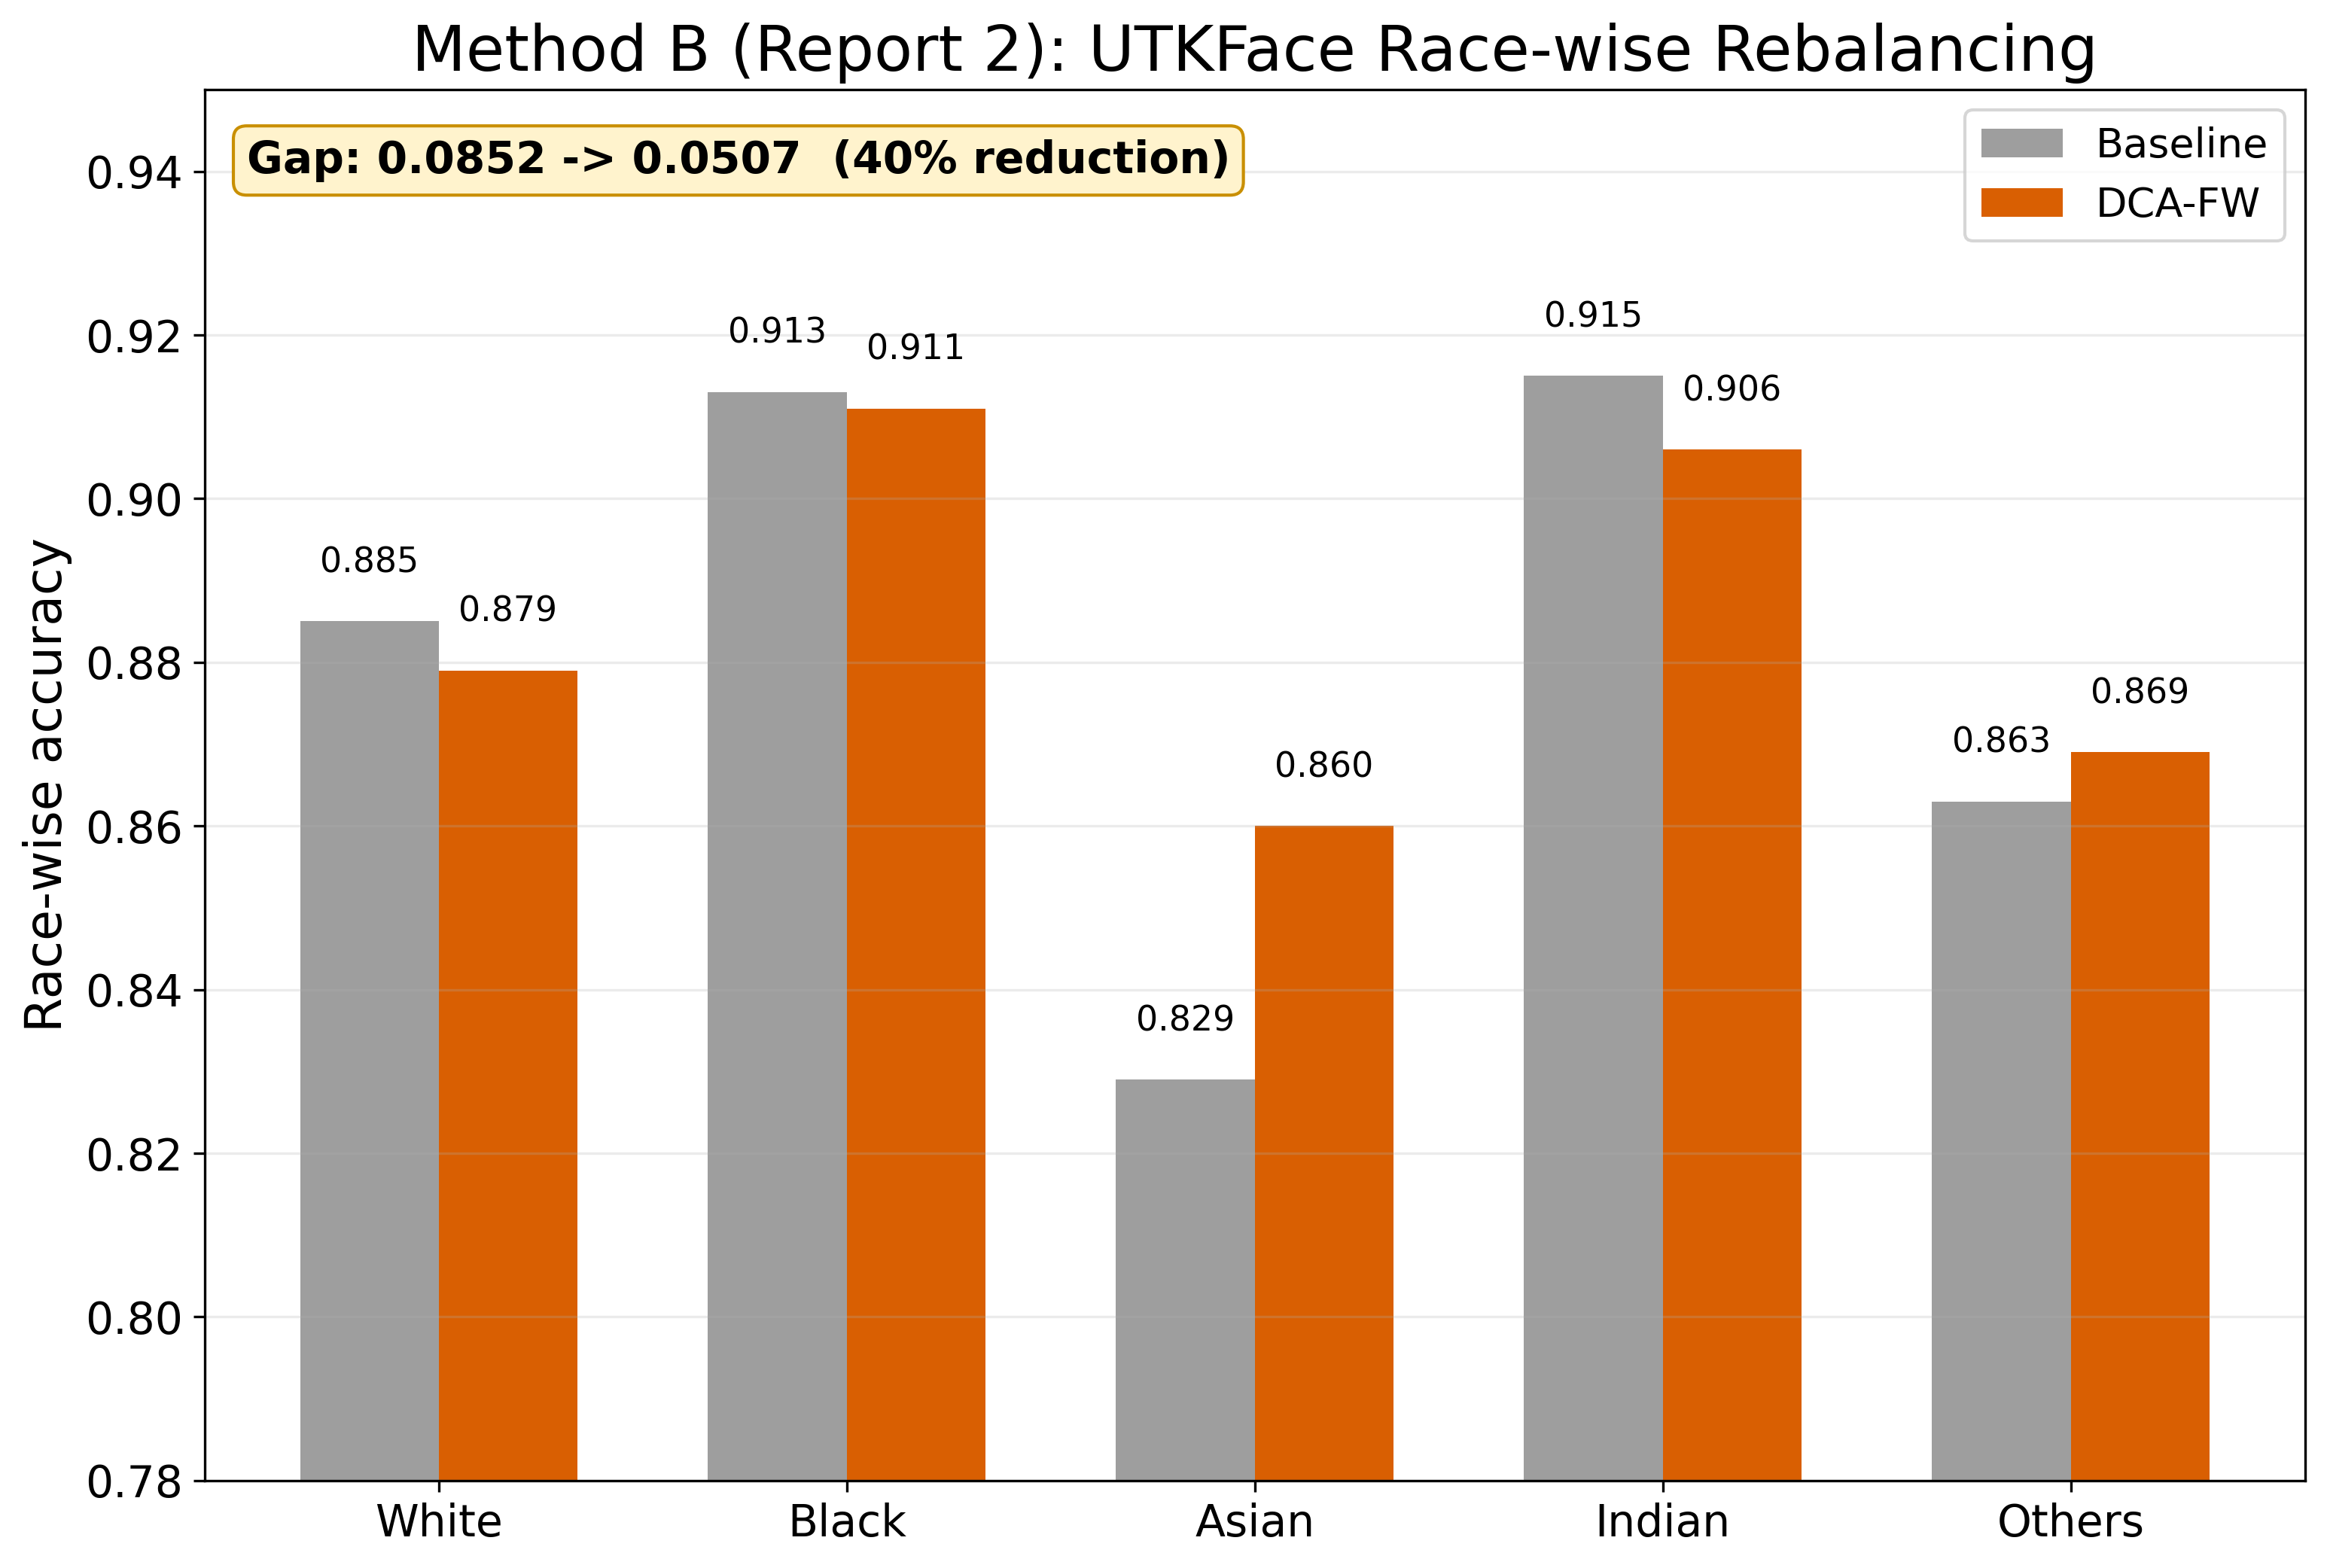
\includegraphics[width=0.97\linewidth]{assets/methodB_race_rebalance.png}}
\end{column}
\begin{column}{0.44\linewidth}
\small
\textbf{Method A Pareto highlights (UTKFace, intervention+protocol)}
\vspace{0.2em}

\begin{tabular}{p{0.52\linewidth}cc}
\toprule
Operating point & Acc & EO \\
\midrule
A2+D2 (IID, AdamW) & 0.9384 & 0.0426 \\
A5+D3 (IID, AdamW) & 0.9345 & 0.0379 \\
A1+D2 (Dir-0.5, AdamW) & 0.9128 & 0.0290 \\
\bottomrule
\end{tabular}

\vspace{0.5em}
\textbf{Method B FairFace validation (Report 2)}

\begin{tabular}{p{0.56\linewidth}cc}
\toprule
Setting & Gap & Acc \\
\midrule
Baseline & 0.0992 & 0.7723 \\
DCA-FW run (40\%) & 0.0880 & 0.7790 \\
DCA-FW run (50\%) & 0.0858 & 0.7695 \\
DCA-FW best-gap run (60\%) & 0.0812 & n/a \\
\bottomrule
\end{tabular}
\end{column}
\end{columns}

\vspace{0.5em}
\begin{columns}[t,totalwidth=\linewidth]
\begin{column}{0.33\linewidth}
\centering
{\fontsize{48}{50}\selectfont\textbf{\color{methodB}{40\%$\downarrow$}}}\\
\Large UTKFace fairness gap (Report 2)
\end{column}
\begin{column}{0.33\linewidth}
\centering
{\fontsize{48}{50}\selectfont\textbf{\color{methodA}{0.9384}}}\\
\Large Best Acc at A2+D2 (Report 1)
\end{column}
\begin{column}{0.33\linewidth}
\centering
{\fontsize{48}{50}\selectfont\textbf{\color{neutralDark}{189}}}\\
\Large Total controlled FL runs (Report 1)
\end{column}
\end{columns}
\end{block}

\UseNeutralBlocks
\begin{columns}[t]

\begin{column}{\sepwid}\end{column}

\begin{column}{\onecolwid}

\begin{block}{Tier 3: Shared Setup and Reading Rule}
\small
\begin{itemize}
\item Task: federated gender classification with race-aware fairness analysis.
\item Common dataset: UTKFace; Report 2 also validates on FairFace.
\item EO/DP (Report 1) and Fairness Gap (Report 2) are complementary fairness views.
\item Interpret fairness gains only at non-degenerate utility levels.
\end{itemize}
\end{block}

\UseMethodBBlocks
\begin{block}{Method B Mechanism (Report 2): DCA-FW}
\small
Client-specific fairness weights are updated from observed race-wise performance,
and then used to reweight local loss in the next round:

\[
w_{k,r}^{(t+1)} = \frac{1}{a_{k,r}^{(t)} + \epsilon},
\qquad
\mathcal{L}_{k}^{(t+1)} = \sum_{r} w_{k,r}^{(t+1)}\,\mathcal{L}_{k,r}
\]

This report-level mechanism is what drives the observed 40\% fairness-gap reduction
on UTKFace while preserving accuracy.
\end{block}

\UseNeutralBlocks
\begin{block}{Contact and Artifacts}
\small
\textbf{Kshitish Kiran Madbhavi} -- kshitish.madbhavi@iitgn.ac.in\\
\textbf{Yash Goyal} -- yash.g@iitgn.ac.in\\
Project guidance: Prof. Manisha Padala

\vspace{0.6em}
\begin{columns}[t,totalwidth=\linewidth]
\begin{column}{0.56\linewidth}
\centering

\includegraphics[width=0.98\linewidth]{iitgn_logo.png}
\end{column}
\begin{column}{0.40\linewidth}
\centering

\includegraphics[width=0.95\linewidth]{contact_qr.png}\\
\scriptsize Scan to request code/data bundle.
\end{column}
\end{columns}
\end{block}

\end{column}

\begin{column}{\sepwid}\end{column}

\begin{column}{\twocolwid}

\UseMethodABlocks
\begin{block}{Tier 2: Figure 1 -- High-Contrast Intervention--Protocol Matrix (Report 1)}
\centering
\fcolorbox{methodA}{white}{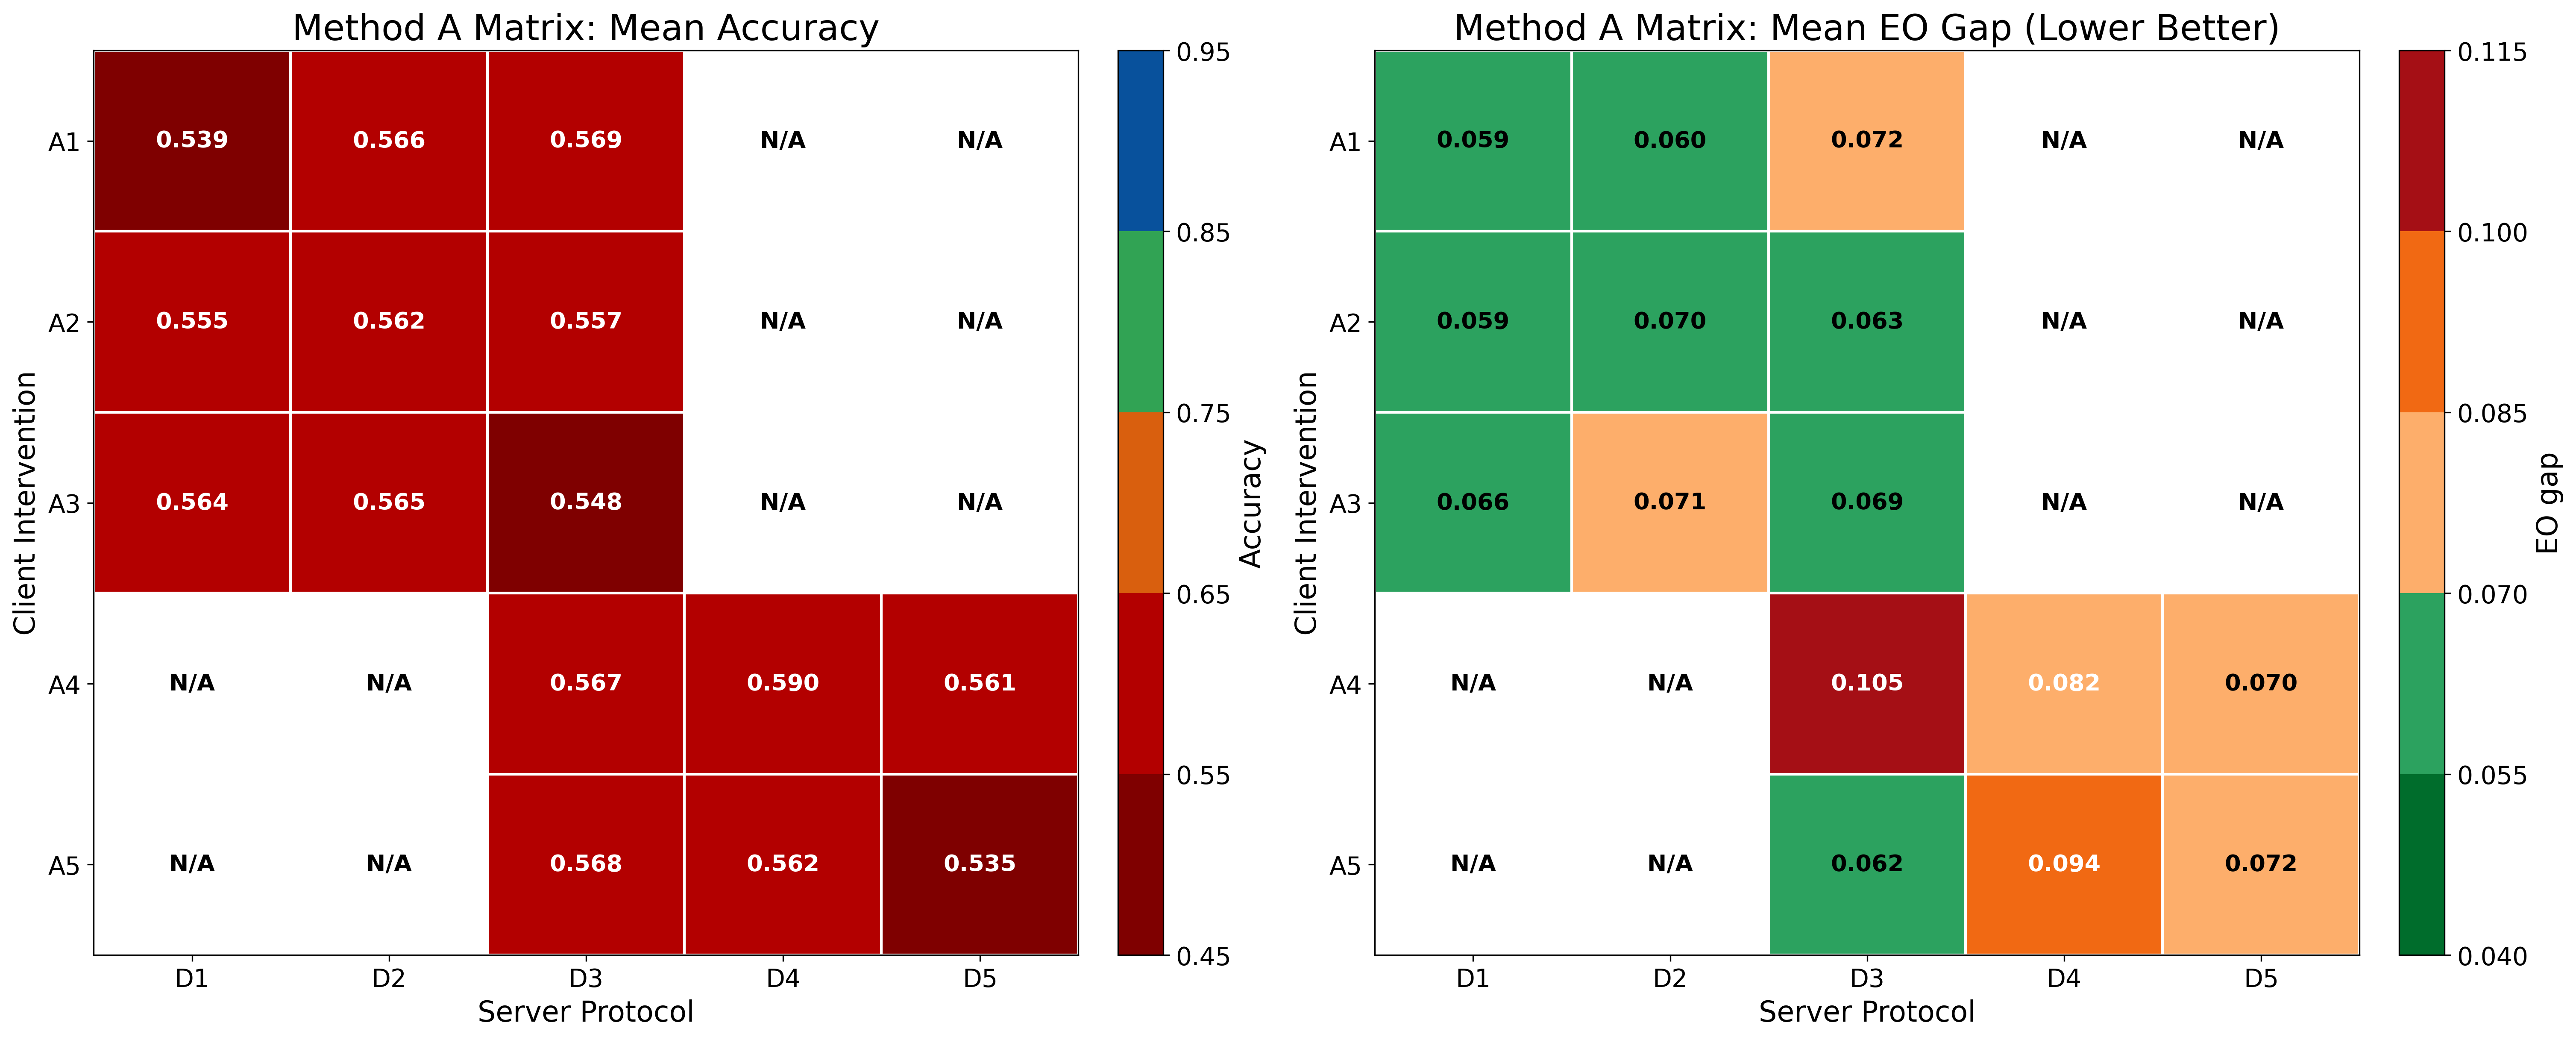
\includegraphics[width=0.98\linewidth]{assets/methodA_matrix_poster.png}}

\small
Matrix cells report mean values across split $\times$ optimizer; unsupported
pairings are explicitly marked as n/a.
\end{block}

\UseMethodABlocks
\begin{block}{Tier 2: Figure 2 -- Pareto Frontier with Best Operating Point (Report 1)}
\centering
\fcolorbox{methodA}{white}{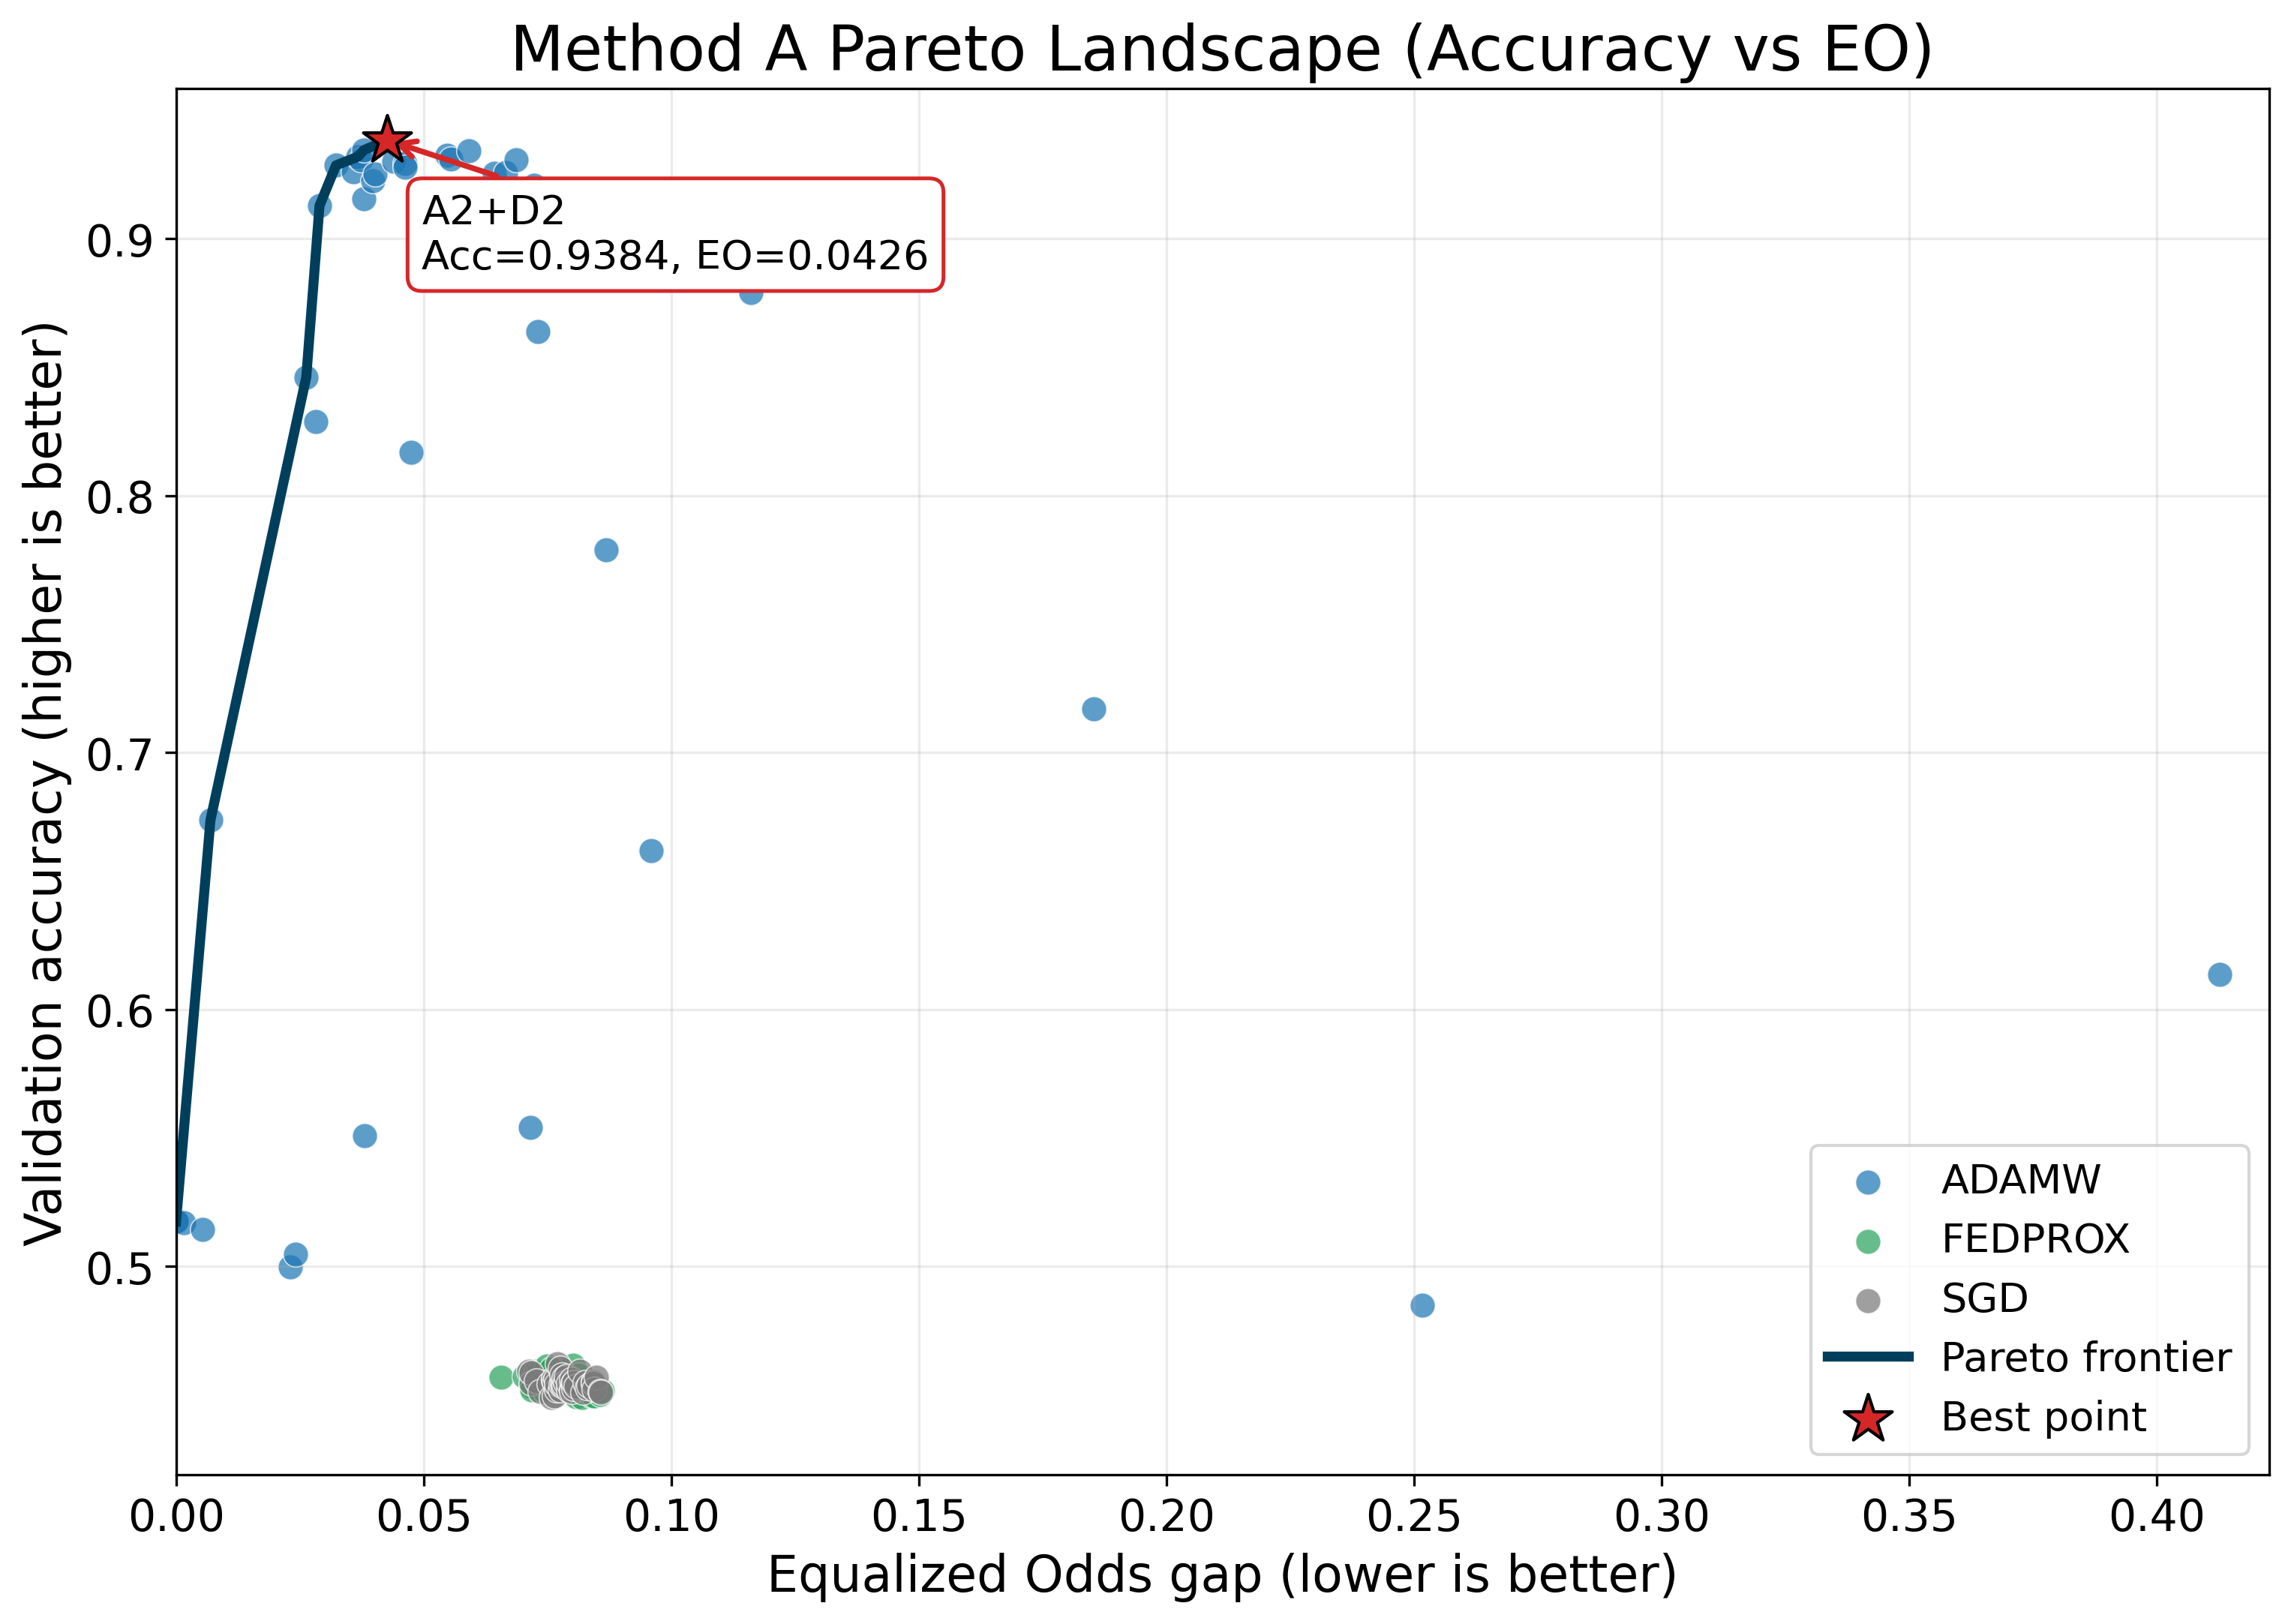
\includegraphics[width=0.98\linewidth]{assets/methodA_pareto_highlight.png}}

\small
The frontier and coordinate annotation show where utility and EO can be jointly optimized.
\end{block}

\end{column}

\begin{column}{\sepwid}\end{column}

\begin{column}{\onecolwid}

\UseNeutralBlocks
\begin{block}{Cross-Method Integration Pipeline}
\centering
\begin{tikzpicture}[>=latex]
\node[draw, rounded corners, fill=methodB!12, text width=0.84\linewidth, align=center] (m2) at (0,0)
{\textbf{Report 2 layer}\\Client-level adaptive fairness weighting (DCA-FW)};
\node[draw, rounded corners, fill=methodA!12, text width=0.84\linewidth, align=center] (m1) at (0,-2.4)
{\textbf{Report 1 layer}\\Server protocol auditing + optimizer-aware governance};
\node[draw, rounded corners, fill=deployBg, text width=0.84\linewidth, align=center] (out) at (0,-4.8)
{\textbf{Deployment target}\\Lower disparity without utility collapse};
\draw[->, very thick, color=methodB] (m2) -- (m1);
\draw[->, very thick, color=methodA] (m1) -- (out);
\end{tikzpicture}
\end{block}

\UseNeutralBlocks
\begin{block}{Tier 3: Limitations and Next Step}
\small
\begin{itemize}
\item Report 1 uses one seed for the 189-run profile.
\item Report 2 includes one FairFace best-gap run with missing accuracy log.
\item Next step: unified multi-seed benchmark where DCA-FW and protocol auditing are co-evaluated in one training stack.
\end{itemize}
\end{block}

\UseNeutralBlocks
\begin{block}{Deployment Recommendations}
\small
\textbf{1. Audit all metrics:} track EO, DP, and Fairness Gap together.\\
\textbf{2. Enable adaptivity:} activate client-level reweighting when race-wise gaps rise.\\
\textbf{3. Guard utility:} keep protocol checks that prevent low-accuracy degenerate zones.\\
\textbf{4. Stress-test shifts:} validate under IID, Dir-0.5, and strict non-IID.
\end{block}

\end{column}

\begin{column}{\sepwid}\end{column}

\end{columns}

\end{frame}

\end{document}
